\begin{frame}{Conversion-node entfernung (if)}

\begin{columns}
	\begin{column}{0.5\textwidth}
		\textbf{Idee:}
		\begin{enumerate}
			\item Entfernen der Conv knoten
			\item Unterstützung anderer Analysen
		\end{enumerate}
		\textbf{Voraussetzung:}
		\begin{enumerate}
			\item Cmp-node mit Const-node und Conv-node
			\item Used bits von Conv-node muss unverändert sein
		\end{enumerate}
	\end{column}
	\begin{column}{0.5\textwidth}  %%<--- here
		\begin{center}
		   \begin{figure}
	\centering
	\begin{tikzpicture}[scale=.7]
		\node[inner sep=0pt] (russell) at (0,0){
			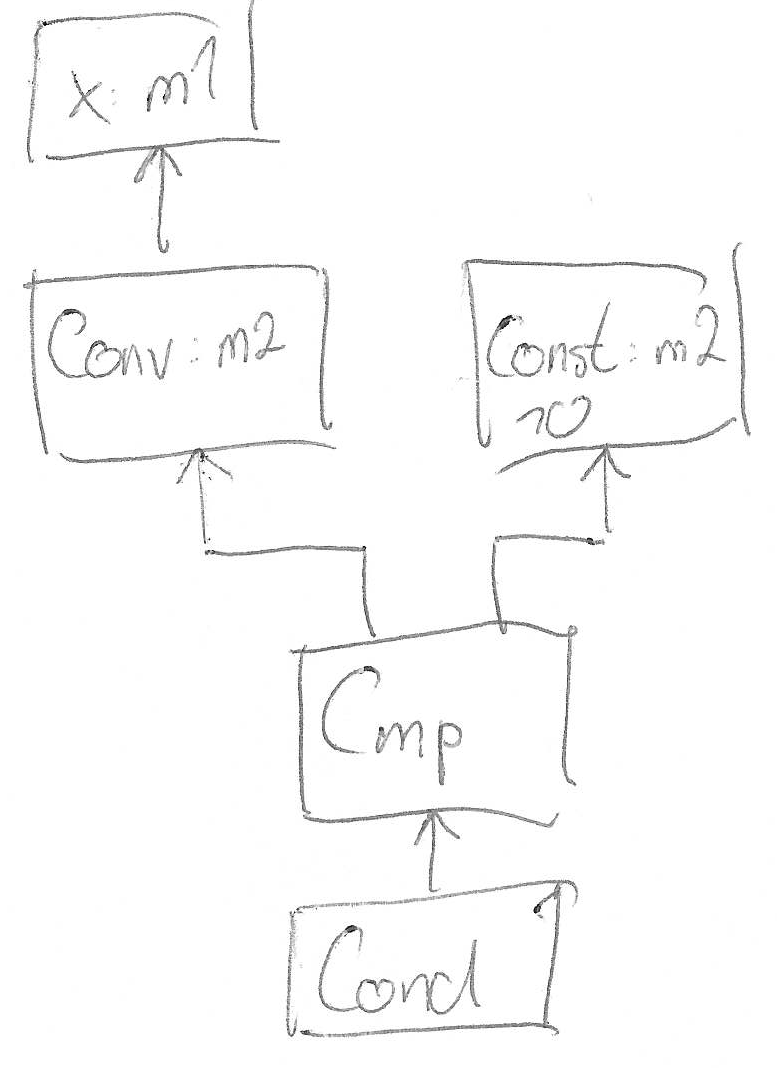
\includegraphics[width=.25\textwidth]{fig/conversion_opt.png}
		};
	\end{tikzpicture}
\caption{Conversion compare construction}
\label{fig:example:conversion_opt}
\end{figure}
		\end{center}
	\end{column}
\end{columns}
\end{frame}

\begin{frame}{Conversion-node entfernung (if)}

\begin{columns}
	\begin{column}{0.5\textwidth}
		\textbf{Optimierung:}
		\begin{enumerate}
			\item Conv-node entfernen
			\item mode von Const anpassen
		\end{enumerate}
	\end{column}
	\begin{column}{0.5\textwidth}  %%<--- here
		\begin{center}
			FIXME
		\end{center}
	\end{column}
\end{columns}
\end{frame}